\begin{frame}{Πειραματική αξιολόγηση: διάταξη}

\begin{minipage}{\linewidth}
  \begin{minipage}{0.3\linewidth}
    \begin{figure}
      % GNUPLOT: LaTeX picture with Postscript
\begingroup
  \makeatletter
  \providecommand\color[2][]{%
    \GenericError{(gnuplot) \space\space\space\@spaces}{%
      Package color not loaded in conjunction with
      terminal option `colourtext'%
    }{See the gnuplot documentation for explanation.%
    }{Either use 'blacktext' in gnuplot or load the package
      color.sty in LaTeX.}%
    \renewcommand\color[2][]{}%
  }%
  \providecommand\includegraphics[2][]{%
    \GenericError{(gnuplot) \space\space\space\@spaces}{%
      Package graphicx or graphics not loaded%
    }{See the gnuplot documentation for explanation.%
    }{The gnuplot epslatex terminal needs graphicx.sty or graphics.sty.}%
    \renewcommand\includegraphics[2][]{}%
  }%
  \providecommand\rotatebox[2]{#2}%
  \@ifundefined{ifGPcolor}{%
    \newif\ifGPcolor
    \GPcolorfalse
  }{}%
  \@ifundefined{ifGPblacktext}{%
    \newif\ifGPblacktext
    \GPblacktexttrue
  }{}%
  % define a \g@addto@macro without @ in the name:
  \let\gplgaddtomacro\g@addto@macro
  % define empty templates for all commands taking text:
  \gdef\gplfronttext{}%
  \gdef\gplfronttext{}%
  \makeatother
  \ifGPblacktext
    % no textcolor at all
    \def\colorrgb#1{}%
    \def\colorgray#1{}%
  \else
    % gray or color?
    \ifGPcolor
      \def\colorrgb#1{\color[rgb]{#1}}%
      \def\colorgray#1{\color[gray]{#1}}%
      \expandafter\def\csname LTw\endcsname{\color{white}}%
      \expandafter\def\csname LTb\endcsname{\color{black}}%
      \expandafter\def\csname LTa\endcsname{\color{black}}%
      \expandafter\def\csname LT0\endcsname{\color[rgb]{1,0,0}}%
      \expandafter\def\csname LT1\endcsname{\color[rgb]{0,1,0}}%
      \expandafter\def\csname LT2\endcsname{\color[rgb]{0,0,1}}%
      \expandafter\def\csname LT3\endcsname{\color[rgb]{1,0,1}}%
      \expandafter\def\csname LT4\endcsname{\color[rgb]{0,1,1}}%
      \expandafter\def\csname LT5\endcsname{\color[rgb]{1,1,0}}%
      \expandafter\def\csname LT6\endcsname{\color[rgb]{0,0,0}}%
      \expandafter\def\csname LT7\endcsname{\color[rgb]{1,0.3,0}}%
      \expandafter\def\csname LT8\endcsname{\color[rgb]{0.5,0.5,0.5}}%
    \else
      % gray
      \def\colorrgb#1{\color{black}}%
      \def\colorgray#1{\color[gray]{#1}}%
      \expandafter\def\csname LTw\endcsname{\color{white}}%
      \expandafter\def\csname LTb\endcsname{\color{black}}%
      \expandafter\def\csname LTa\endcsname{\color{black}}%
      \expandafter\def\csname LT0\endcsname{\color{black}}%
      \expandafter\def\csname LT1\endcsname{\color{black}}%
      \expandafter\def\csname LT2\endcsname{\color{black}}%
      \expandafter\def\csname LT3\endcsname{\color{black}}%
      \expandafter\def\csname LT4\endcsname{\color{black}}%
      \expandafter\def\csname LT5\endcsname{\color{black}}%
      \expandafter\def\csname LT6\endcsname{\color{black}}%
      \expandafter\def\csname LT7\endcsname{\color{black}}%
      \expandafter\def\csname LT8\endcsname{\color{black}}%
    \fi
  \fi
  \setlength{\unitlength}{0.02500bp}%
  \begin{picture}(4000.00,4000.00)%
    \gplgaddtomacro\gplfronttext{%
      \colorrgb{0.00,0.00,0.00}%
      \put(388,778){\makebox(0,0)[r]{\strut{}\footnotesize $4$}}%
      \colorrgb{0.00,0.00,0.00}%
      \put(388,1295){\makebox(0,0)[r]{\strut{}\footnotesize $6$}}%
      \colorrgb{0.00,0.00,0.00}%
      \put(388,1811){\makebox(0,0)[r]{\strut{}\footnotesize $8$}}%
      \colorrgb{0.00,0.00,0.00}%
      \put(388,2328){\makebox(0,0)[r]{\strut{}\footnotesize $10$}}%
      \colorrgb{0.00,0.00,0.00}%
      \put(388,2844){\makebox(0,0)[r]{\strut{}\footnotesize $12$}}%
      \colorrgb{0.00,0.00,0.00}%
      \put(388,3361){\makebox(0,0)[r]{\strut{}\footnotesize $14$}}%
      \colorrgb{0.00,0.00,0.00}%
      \put(778,300){\makebox(0,0){\strut{}\footnotesize $4$}}%
      \colorrgb{0.00,0.00,0.00}%
      \put(1295,300){\makebox(0,0){\strut{}\footnotesize $6$}}%
      \colorrgb{0.00,0.00,0.00}%
      \put(1811,300){\makebox(0,0){\strut{}\footnotesize $8$}}%
      \colorrgb{0.00,0.00,0.00}%
      \put(2328,300){\makebox(0,0){\strut{}\footnotesize $10$}}%
      \colorrgb{0.00,0.00,0.00}%
      \put(2844,300){\makebox(0,0){\strut{}\footnotesize $12$}}%
      \colorrgb{0.00,0.00,0.00}%
      \put(3361,300){\makebox(0,0){\strut{}\footnotesize $14$}}%
      \colorrgb{0.00,0.00,0.00}%
      \put(-318,2069){\rotatebox{90}{\makebox(0,0){\strut{}$y$ [m]}}}%
      \colorrgb{0.00,0.00,0.00}%
      \put(2069,-230){\makebox(0,0){\strut{}$x$ [m]}}%
    }%
    \gplgaddtomacro\gplfronttext{%
    }%
    \put(0,0){
\includegraphics[scale=0.5]{./figures/slides/ch3/corridor}}%
    \gplfronttext
  \end{picture}%
\endgroup

      \vspace{0.5cm}
      \caption{\small Χάρτης $\bm{M}_C$}
    \end{figure}
  \end{minipage}
  \begin{minipage}{0.3\linewidth}
    \begin{figure}
      % GNUPLOT: LaTeX picture with Postscript
\begingroup
  \makeatletter
  \providecommand\color[2][]{%
    \GenericError{(gnuplot) \space\space\space\@spaces}{%
      Package color not loaded in conjunction with
      terminal option `colourtext'%
    }{See the gnuplot documentation for explanation.%
    }{Either use 'blacktext' in gnuplot or load the package
      color.sty in LaTeX.}%
    \renewcommand\color[2][]{}%
  }%
  \providecommand\includegraphics[2][]{%
    \GenericError{(gnuplot) \space\space\space\@spaces}{%
      Package graphicx or graphics not loaded%
    }{See the gnuplot documentation for explanation.%
    }{The gnuplot epslatex terminal needs graphicx.sty or graphics.sty.}%
    \renewcommand\includegraphics[2][]{}%
  }%
  \providecommand\rotatebox[2]{#2}%
  \@ifundefined{ifGPcolor}{%
    \newif\ifGPcolor
    \GPcolorfalse
  }{}%
  \@ifundefined{ifGPblacktext}{%
    \newif\ifGPblacktext
    \GPblacktexttrue
  }{}%
  % define a \g@addto@macro without @ in the name:
  \let\gplgaddtomacro\g@addto@macro
  % define empty templates for all commands taking text:
  \gdef\gplfronttext{}%
  \gdef\gplfronttext{}%
  \makeatother
  \ifGPblacktext
    % no textcolor at all
    \def\colorrgb#1{}%
    \def\colorgray#1{}%
  \else
    % gray or color?
    \ifGPcolor
      \def\colorrgb#1{\color[rgb]{#1}}%
      \def\colorgray#1{\color[gray]{#1}}%
      \expandafter\def\csname LTw\endcsname{\color{white}}%
      \expandafter\def\csname LTb\endcsname{\color{black}}%
      \expandafter\def\csname LTa\endcsname{\color{black}}%
      \expandafter\def\csname LT0\endcsname{\color[rgb]{1,0,0}}%
      \expandafter\def\csname LT1\endcsname{\color[rgb]{0,1,0}}%
      \expandafter\def\csname LT2\endcsname{\color[rgb]{0,0,1}}%
      \expandafter\def\csname LT3\endcsname{\color[rgb]{1,0,1}}%
      \expandafter\def\csname LT4\endcsname{\color[rgb]{0,1,1}}%
      \expandafter\def\csname LT5\endcsname{\color[rgb]{1,1,0}}%
      \expandafter\def\csname LT6\endcsname{\color[rgb]{0,0,0}}%
      \expandafter\def\csname LT7\endcsname{\color[rgb]{1,0.3,0}}%
      \expandafter\def\csname LT8\endcsname{\color[rgb]{0.5,0.5,0.5}}%
    \else
      % gray
      \def\colorrgb#1{\color{black}}%
      \def\colorgray#1{\color[gray]{#1}}%
      \expandafter\def\csname LTw\endcsname{\color{white}}%
      \expandafter\def\csname LTb\endcsname{\color{black}}%
      \expandafter\def\csname LTa\endcsname{\color{black}}%
      \expandafter\def\csname LT0\endcsname{\color{black}}%
      \expandafter\def\csname LT1\endcsname{\color{black}}%
      \expandafter\def\csname LT2\endcsname{\color{black}}%
      \expandafter\def\csname LT3\endcsname{\color{black}}%
      \expandafter\def\csname LT4\endcsname{\color{black}}%
      \expandafter\def\csname LT5\endcsname{\color{black}}%
      \expandafter\def\csname LT6\endcsname{\color{black}}%
      \expandafter\def\csname LT7\endcsname{\color{black}}%
      \expandafter\def\csname LT8\endcsname{\color{black}}%
    \fi
  \fi
  \setlength{\unitlength}{0.0500bp}%
  \begin{picture}(3000.00,6000.00)%
    \gplgaddtomacro\gplfronttext{%
      \colorrgb{0.00,0.00,0.00}%
      \put(340,977){\makebox(0,0)[r]{\strut{}$45$}}%
      \colorrgb{0.00,0.00,0.00}%
      \put(340,1612){\makebox(0,0)[r]{\strut{}$50$}}%
      \colorrgb{0.00,0.00,0.00}%
      \put(340,2247){\makebox(0,0)[r]{\strut{}$55$}}%
      \colorrgb{0.00,0.00,0.00}%
      \put(340,2882){\makebox(0,0)[r]{\strut{}$60$}}%
      \colorrgb{0.00,0.00,0.00}%
      \put(340,3517){\makebox(0,0)[r]{\strut{}$65$}}%
      \colorrgb{0.00,0.00,0.00}%
      \put(340,4152){\makebox(0,0)[r]{\strut{}$70$}}%
      \colorrgb{0.00,0.00,0.00}%
      \put(340,4787){\makebox(0,0)[r]{\strut{}$75$}}%
      \colorrgb{0.00,0.00,0.00}%
      \put(340,5422){\makebox(0,0)[r]{\strut{}$80$}}%
      \colorrgb{0.00,0.00,0.00}%
      \put(536,440){\makebox(0,0){\strut{}$56$}}%
      \colorrgb{0.00,0.00,0.00}%
      \put(1044,440){\makebox(0,0){\strut{}$60$}}%
      \colorrgb{0.00,0.00,0.00}%
      \put(1679,440){\makebox(0,0){\strut{}$65$}}%
      \colorrgb{0.00,0.00,0.00}%
      \put(2314,440){\makebox(0,0){\strut{}$70$}}%
      \colorrgb{0.00,0.00,0.00}%
      \put(-166,3104){\rotatebox{90}{\makebox(0,0){\strut{}$y$ [m]}}}%
      \colorrgb{0.00,0.00,0.00}%
      \put(1551,110){\makebox(0,0){\strut{}$x$ [m]}}%
    }%
    \gplgaddtomacro\gplfronttext{%
    }%
    \put(0,0){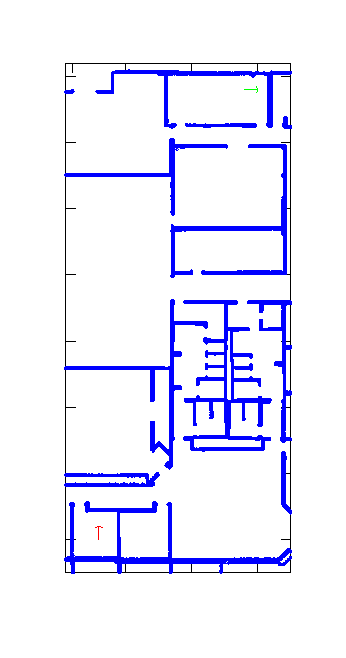
\includegraphics{./figures/parts/02/chapters/01/sections/03/willowgarage}}%
    \gplfronttext
  \end{picture}%
\endgroup

      \vspace{0.25cm}
      \caption{\small Χάρτης $\bm{M}_W$}
    \end{figure}
  \end{minipage}
  \begin{minipage}{0.3\linewidth}
    \begin{figure}
      % GNUPLOT: LaTeX picture with Postscript
\begingroup
  \makeatletter
  \providecommand\color[2][]{%
    \GenericError{(gnuplot) \space\space\space\@spaces}{%
      Package color not loaded in conjunction with
      terminal option `colourtext'%
    }{See the gnuplot documentation for explanation.%
    }{Either use 'blacktext' in gnuplot or load the package
      color.sty in LaTeX.}%
    \renewcommand\color[2][]{}%
  }%
  \providecommand\includegraphics[2][]{%
    \GenericError{(gnuplot) \space\space\space\@spaces}{%
      Package graphicx or graphics not loaded%
    }{See the gnuplot documentation for explanation.%
    }{The gnuplot epslatex terminal needs graphicx.sty or graphics.sty.}%
    \renewcommand\includegraphics[2][]{}%
  }%
  \providecommand\rotatebox[2]{#2}%
  \@ifundefined{ifGPcolor}{%
    \newif\ifGPcolor
    \GPcolorfalse
  }{}%
  \@ifundefined{ifGPblacktext}{%
    \newif\ifGPblacktext
    \GPblacktexttrue
  }{}%
  % define a \g@addto@macro without @ in the name:
  \let\gplgaddtomacro\g@addto@macro
  % define empty templates for all commands taking text:
  \gdef\gplfronttext{}%
  \gdef\gplfronttext{}%
  \makeatother
  \ifGPblacktext
    % no textcolor at all
    \def\colorrgb#1{}%
    \def\colorgray#1{}%
  \else
    % gray or color?
    \ifGPcolor
      \def\colorrgb#1{\color[rgb]{#1}}%
      \def\colorgray#1{\color[gray]{#1}}%
      \expandafter\def\csname LTw\endcsname{\color{white}}%
      \expandafter\def\csname LTb\endcsname{\color{black}}%
      \expandafter\def\csname LTa\endcsname{\color{black}}%
      \expandafter\def\csname LT0\endcsname{\color[rgb]{1,0,0}}%
      \expandafter\def\csname LT1\endcsname{\color[rgb]{0,1,0}}%
      \expandafter\def\csname LT2\endcsname{\color[rgb]{0,0,1}}%
      \expandafter\def\csname LT3\endcsname{\color[rgb]{1,0,1}}%
      \expandafter\def\csname LT4\endcsname{\color[rgb]{0,1,1}}%
      \expandafter\def\csname LT5\endcsname{\color[rgb]{1,1,0}}%
      \expandafter\def\csname LT6\endcsname{\color[rgb]{0,0,0}}%
      \expandafter\def\csname LT7\endcsname{\color[rgb]{1,0.3,0}}%
      \expandafter\def\csname LT8\endcsname{\color[rgb]{0.5,0.5,0.5}}%
    \else
      % gray
      \def\colorrgb#1{\color{black}}%
      \def\colorgray#1{\color[gray]{#1}}%
      \expandafter\def\csname LTw\endcsname{\color{white}}%
      \expandafter\def\csname LTb\endcsname{\color{black}}%
      \expandafter\def\csname LTa\endcsname{\color{black}}%
      \expandafter\def\csname LT0\endcsname{\color{black}}%
      \expandafter\def\csname LT1\endcsname{\color{black}}%
      \expandafter\def\csname LT2\endcsname{\color{black}}%
      \expandafter\def\csname LT3\endcsname{\color{black}}%
      \expandafter\def\csname LT4\endcsname{\color{black}}%
      \expandafter\def\csname LT5\endcsname{\color{black}}%
      \expandafter\def\csname LT6\endcsname{\color{black}}%
      \expandafter\def\csname LT7\endcsname{\color{black}}%
      \expandafter\def\csname LT8\endcsname{\color{black}}%
    \fi
  \fi
  \setlength{\unitlength}{0.0400bp}%
  \begin{picture}(4000.00,4000.00)%
    \gplgaddtomacro\gplfronttext{%
      \colorrgb{0.00,0.00,0.00}%
      \put(388,793){\makebox(0,0)[r]{\strut{}\footnotesize $0$}}%
      \colorrgb{0.00,0.00,0.00}%
      \put(388,1158){\makebox(0,0)[r]{\strut{}\footnotesize $2$}}%
      \colorrgb{0.00,0.00,0.00}%
      \put(388,1522){\makebox(0,0)[r]{\strut{}\footnotesize $4$}}%
      \colorrgb{0.00,0.00,0.00}%
      \put(388,1887){\makebox(0,0)[r]{\strut{}\footnotesize $6$}}%
      \colorrgb{0.00,0.00,0.00}%
      \put(388,2251){\makebox(0,0)[r]{\strut{}\footnotesize $8$}}%
      \colorrgb{0.00,0.00,0.00}%
      \put(388,2616){\makebox(0,0)[r]{\strut{}\footnotesize $10$}}%
      \colorrgb{0.00,0.00,0.00}%
      \put(388,2980){\makebox(0,0)[r]{\strut{}\footnotesize $12$}}%
      \colorrgb{0.00,0.00,0.00}%
      \put(388,3345){\makebox(0,0)[r]{\strut{}\footnotesize $14$}}%
      \colorrgb{0.00,0.00,0.00}%
      \put(520,573){\makebox(0,0){\strut{}\footnotesize $6$}}%
      \colorrgb{0.00,0.00,0.00}%
      \put(885,573){\makebox(0,0){\strut{}\footnotesize $8$}}%
      \colorrgb{0.00,0.00,0.00}%
      \put(1249,573){\makebox(0,0){\strut{}\footnotesize $10$}}%
      \colorrgb{0.00,0.00,0.00}%
      \put(1614,573){\makebox(0,0){\strut{}\footnotesize $12$}}%
      \colorrgb{0.00,0.00,0.00}%
      \put(1978,573){\makebox(0,0){\strut{}\footnotesize $14$}}%
      \colorrgb{0.00,0.00,0.00}%
      \put(2343,573){\makebox(0,0){\strut{}\footnotesize $16$}}%
      \colorrgb{0.00,0.00,0.00}%
      \put(2708,573){\makebox(0,0){\strut{}\footnotesize $18$}}%
      \colorrgb{0.00,0.00,0.00}%
      \put(3072,573){\makebox(0,0){\strut{}\footnotesize $20$}}%
      \colorrgb{0.00,0.00,0.00}%
      \put(3437,573){\makebox(0,0){\strut{}\footnotesize $22$}}%
      \colorrgb{0.00,0.00,0.00}%
      \put(-118,2069){\rotatebox{90}{\makebox(0,0){\strut{}$y$ [m]}}}%
      \colorrgb{0.00,0.00,0.00}%
      \put(2069,243){\makebox(0,0){\strut{}$x$ [m]}}%
    }%
    \gplgaddtomacro\gplfronttext{%
    }%
    \put(0,0){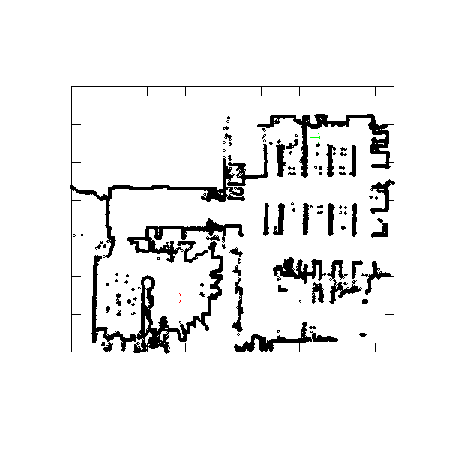
\includegraphics[scale=0.8]{./figures/slides/ch3/csal}}%
    \gplfronttext
  \end{picture}%
\endgroup

      \caption{\small Χάρτης $\bm{M}_L$}
    \end{figure}
  \end{minipage}
\end{minipage}

\note{\footnotesize Η αξιολόγηση κάθε συνδυασμού έγινε σε δύο περιβάλλοντα
  προσομοίωσης και σε ένα πραγματικό περιβάλλον. Και στις τρεις περιπτώσεις
  θέσαμε μία αρχική και μία τελική στάση και ζητήσαμε από κάθε συνδυασμό global
  και local planners να πλοηγηθεί αυτόνομα από την αρχική στην τελική στάση με
  βάση το μονοπάτι που θα σχεδίαζε ο global planner και τις εντολές κίνησης του
  local planner. Κάθε συνδυασμός απο planners επανέλαβε το πείραμα 10 φορές σε
  κάθε περιβάλλον, και για κάθε πείραμα καταγράφηκε ένας αριθμός από μετρικές
  προκειμένου να γίνει η αξιολόγηση κάθε συνδυασμού και να υπάρχει ένα κοινό
  σύστημα κρίσης για όλους ώστε στο τέλος να προκύψει μία ιεραρχία συνδυασμών.}

\end{frame}
